
\section{Proposal}
\label{sec:proposal}

In this section, we present \RPCBROADCAST, a causal broadcast protocol removing
the last linear upper bound in terms of number of processes that ever broadcast
a message that remained on space complexity. \RPCBROADCAST exploits the
improvement brought by \PCBROADCAST on generated traffic to reduce the space
consumed by reliable broadcast, at marginal cost.

\subsection{Model}

A distributed system comprises a set of processes that can communicate with each
other using messages. Processes may not have full knowledge of the membership of
the system. Instead, processes build and maintain overlay networks: each process
updates a local partial view of logical communication channels, i.e., a set of
processes to communicate with. The partial view is usually much smaller than the
actual system size. We speak of overlay networks, networks, or distributed
systems indifferently.

\begin{definition}[Overlay network]
  An overlay network comprises a set of processes that run a set of instructions
  sequentially.  An overlay network also comprises a set of directed
  links. \\
  An overlay network is dynamic if the set of processes or the set of links is
  mutable. Otherwise, the overlay network is static. \\
  The set of links departing from a process is its neighborhood, or partial
  view, or out-view. The set of links arriving to a process is its in-view. \\
  A link from a process to another process allows the former to transmit
  information to the latter. Processes transmit information using asynchronous
  message passing.\\
  Processes are faulty if they crash, otherwise they are correct. There are no
  byzantine processes.
\end{definition}

Processes can communicate with each other using message passing. Process~A can
send a message $m$ to Process~B $s_{AB}(m)$. Process~A can receive a message $m$
from another process B $r_{AB}(m)$, or from any other process
$r_A(m)$. Process~A can send a message $m$ to all other processes of the system,
i.e., it broadcasts a message $b_A(m)$. Process~A can deliver a message
$d_A(m)$.

To characterize the order among events such as send, or receive, we define time
in a logical sense using Lamport’s definition.

\begin{definition}[Happen before~\cite{lamport1978time}]
  Happen before is a transitive, irreflexive, and antisymmetric relation that
  defines a strict partial orders of events. The sending of a message always
  precedes its receipt $s_{AB}(m) \rightarrow r_{BA}(m)$. Two messages are
  concurrent if none happens before the other.
\end{definition}

\begin{definition}[Uniform reliable broadcast] 
  When a process broadcasts a message to all processes of the network, correct
  processes eventually receive it. Uniform reliable broadcast guarantees 3
  properties:
  \begin{itemize}[leftmargin=*]
  \item Validity: If a correct process broadcasts a message, then it
    eventually delivers it.
  \item Uniform Agreement: If a process -- correct or not -- delivers a message,
    then all correct processes eventually deliver it.
  \item Uniform Integrity: A process delivers a message at most once, and only if
    it was previously broadcast.
  \end{itemize}
\end{definition}

From uniform integrity, we derive that despite multiple receipts, a process
delivers a message once.

\begin{definition}[Exactly once delivery]
  Each process receives each broadcast message at least once. A process may
  \begin{enumerate}
  \item $\forall A,\,B,\, b_A(m) \implies r_B(m)$
  \item $\forall m,\, d_A(m) \implies \exists r_A(m),\, r_A(m) \rightarrow d_A(m)$
  \item \label{enum:uniqueness}
    $\forall m,\,m',\, d_A(m) \rightarrow d_A(m') \implies m \neq m'$
  \end{enumerate}
\end{definition}

Property~\ref{enum:uniqueness} suggests the use of a data structure ensuring
uniqueness of messages such as sets or vectors. The data structure allows
processes to remember about prior receipts of messages in order to discard
double receipts.


\begin{algorithm}[h]
  \SetKwProg{Function}{function}{}{}
\SetKwProg{Upon}{upon}{}{}
\SetKwProg{Initially}{INITIALLY:}{}{}
\SetKwProg{Dissemination}{DISSEMINATION:}{}{}

\small

\DontPrintSemicolon
\LinesNumbered

\Initially {} {
  $Q_o$ \tcp*{Set of processes, $p$'s out-view}
  $Q_i$ \tcp*{Set of processes, $p$'s in-view}
  \BlankLine
  $E \leftarrow \varnothing$ \tcp*{Map of expected messages $Q_i : M^*$}
}

\BlankLine

\Dissemination{}{

%  \begin{multicols}{2}

  \Function{$\textup{R-broadcast}(m)$} { %\tcp*[f]{$b_p(m)$}} { 
    % $\textup{received}(m,\, \_)$ \;
    % \lForEach {$q \in Q_o$} {\textup{sendTo}($q,\, m$)}
    % \textup{R-deliver}($m$) \; % \tcp*{$d_p(m)$}
    $\textup{receive}(m,\, \_)$ \;
  }

  \BlankLine
  
  \Upon{$\textup{receive}(m,\, l)$}{
    \If {$\neg\textup{received}(m,\,l)$} {
      \lForEach {$q \in Q_o$} {\textup{sendTo}($q,\, m$)}
      % \tcp*[f]{broadcast or forward}}
      \textup{R-deliver}($m$) \; % \tcp*{$d_p(m)$}
    }
  }

  \BlankLine
  
  \Function{$\textup{received}(m,\, l)$}{
    \textbf{let} $rcvd \leftarrow
    \exists q \in E$ \textbf{\textup{with}} $m\in E[q]$ \;
    \If {$\neg rcvd$} {
      \ForEach {$q \in Q_i$} {$E[q] \leftarrow E[q] \cup m$ \label{line:remembers}}
        % \tcp*[f]{to remember}}
    }
    $E[l] \leftarrow E[l] \setminus m$ \label{line:forgets} \;%\tcp*{to forget}
    \Return $rcvd$ \;
  }

%  \end{multicols}

%  \BlankLine  
}


%%% Local Variables:
%%% mode: latex
%%% TeX-master: "../paper"
%%% End:

  \caption{\label{algo:reliablebroadcast}R-broadcast at Process $p$.}
\end{algorithm}

Algorithm~\ref{algo:reliablebroadcast} shows the instructions of a uniform
reliable broadcast ensuring uniqueness of delivery in static systems. It
features a data structure that can be safely purged over time. Similarly to
Algorithm~\ref{algo:counterrbroadcast}, it uses the in-view and exploits the
property that each process sends each message exactly once to each neighbor in
their out-view.
% As long as each link did not convey the 
% Each process will receive a copy from each link in its in-view exactly
% once. Afterwards, they purge their structure for they will never receive such
% message again.
Instead of using counters, it associates with each link from the in-view a set
of expected messages. When Process~A receives a message for the first time from
Process~B, it awaits a copy of this message from all other processes in its
in-view. When it receives such copy, it removes the message from the set of
awaited messages of the corresponding link. Process~A will never receive a copy
of this message from this link again. Once it received all awaited copies, it
will never receive a copy of this message at all.
% The principle of this implementation is similar to that of
% Figure~\ref{fig:generalpurge} to which it adds an awareness of links with
% awaited messages. 
Each process remembers each broadcast message as long as it is susceptible to
arrive again.

\begin{definition}[Remember]
  A process remembers a message after its first receipt until its last receipt,
  i.e., once the process received the message from its whole in-view.
  $remember_B(m) \equiv \exists A \in Q_i,\, r_B(m) \wedge \neg r_{BA}(m)$
\end{definition}

\begin{theorem}[Remembering ensures exactly once delivery]
  Delivering broadcast messages when they are not remembered ensures exactly
  once delivery.
  $(\forall m,\, r_B(m) \wedge \neg remember_B(m) \Longleftrightarrow d_B(m))
  \implies (\forall m,\,m',\, d_B(m) \rightarrow d_B(m') \implies m \neq m')$
\end{theorem}

\begin{proof}
  We must show that delivering messages while they are not remembered implies
  uniqueness of delivery. \\ 
  
  Assuming that each process delivers and forwards each broadcast message
  exactly once, each link conveys each broadcast message exactly once.  Each
  link conveys distinct messages:
  $\forall m,\,m' ,\, r_{AB}(m) \rightarrow r_{AB}(m') \implies m \neq m'$.
  
  \TODO{Heeeeere.}
  
  In addition, the first receipt of a message $m$ marks other links in the
  in-view with this awaited message. $\forall m,\, r_AB(m) \implies $

  % In addition, the first receipt by a link marks other links in the in-view.

  
  We must show that a process that forgets a message $m$ before its receipt from
  the whole in-view may deliver it multiple times. \TODO{Not
    enough}. \TODO{Meow.}
\end{proof}

% Using this reliable broadcast implementation, each process delivers each message
% exactly once.

In addition to reliable delivery, broadcast protocols can guarantee a delivery
order of messages. We focus on causal order. Process~A should deliver a message
$m$ from Process~B after having delivered all messages delivered by Process~B
before the sending of $m$.

\begin{definition}[Causal order]
  The delivery order of messages follows the happen before relationships of the
  corresponding broadcasts.
  $d_A(m) \rightarrow b_A(m') \implies d_B(m) \rightarrow d_B(m')$
\end{definition}

\begin{definition}[Causal broadcast]
  Causal broadcast is a uniform reliable broadcast ensuring causal order.
\end{definition}

\PCBROADCAST (\REF) is a causal broadcast that uses FIFO links, control
messages, and buffers to ensure causal order in dynamic systems. A process
broadcasting a message sends the message to an out-view of safe links.

\begin{definition}[\label{def:safe}Safe link] 
  A link from Process~A to Process~B is safe if and only if Process~B received
  or will receive all messages delivered by Process~A before receiving any
  message that Process~A will
  deliver. $safe(AB) \equiv \forall m,\, m',\, d_A(m) \rightarrow s_{AB}(m')
  \implies r_B(m) \rightarrow r_{BA}(m')$
\end{definition}

Links start unsafe, for messages traveling by the new links may arrive before
preceding messages that took longer paths. \PCBROADCAST ensures that they are
safe, i.e., they cannot cause causal order violations, by sending control
messages.

\begin{definition}[Ping phase]
  Ping phase starts when Process~A pings Process~B. Ping messages $\pi$ travel
  using safe links. When Process~B receives this ping, it replies to
  Process~A. Replies $\rho$ travel using any communication mean. Ping phase ends
  when Process~A receives the reply of Process~B.
\end{definition}

\begin{lemma}[\label{lemma:ping}Ping phases acknowledge broadcast receipts]
  A ping phase from Process~A to Process~B acknowledges the receipt by B of all
  messages delivered by Process~A before this ping phase.
  $\forall m,\, d_A(m) \rightarrow s_A(\pi_{AB}) \wedge r_A(\rho_{AB}) \implies
  r_B(m)$
\end{lemma}

\PCBROADCAST ensures that all preceding messages arrive before new messages by
acknowledging the receipt of most messages while buffering messages concurrent
to the acknowledgment.


% \begin{lemma}[Buffer $B$ \TODO{Move, does not make sense here yet}]
%   $\forall m,\, s_A(\pi_{AB}) \rightarrow d_A(m) \wedge d_A(m) \rightarrow r_A(\rho_{AB})
%   \Longleftrightarrow m \in B$
% \end{lemma}

However, this is insufficient to ensure exactly once delivery. The issue is
identical to that depicted in Figure~\ref{fig:generalproblem}. Process~B adds
Process~C in its out-view but Process~C already forgot about the message $a$
while Process~B received it. This leads to double delivery of $a$ and subsequent
inconsistencies.

In this paper, we exploit causal communication to implement a stronger meaning
of safe link at marginal cost. A link becomes safe when it cannot violate both
causal delivery and exactly once delivery.  This is more expensive to ensure in
terms of control messages, for it must account for concurrent messages between
involved processes. The rest of this section describes the operation of our
proposal and its complexity.

%broadcast requires more ping phases and
%more buffers.


\subsection{Operation}


\begin{algorithm}[h]
  \SetKwProg{Function}{function}{}{}
\SetKwProg{Upon}{upon}{}{}
\SetKwProg{Initially}{INITIALLY:}{}{}
\SetKwProg{Safety}{SAFETY:}{}{}
\SetKwProg{Dissemination}{DISSEMINATION:}{}{}

\SetKwComment{EmptyComment}{}{}

\small

\DontPrintSemicolon
\LinesNumbered

%\begin{multicols}{2}
\Initially {} {
%  $Q_o$ \tcp*{Set of processes, $p$'s outview}
%  $Q_i$ \tcp*{Set of processes, $p$'s inview}
%  \BlankLine  
  $B \leftarrow \varnothing$ \tcp*{$@$Sender Map of buffers $Q_o : M^*$}
%  \BlankLine  
  $S \leftarrow \varnothing$ \tcp*{$@$Receiver Map of buffers $Q_i : M^* \times M^* \times bool$}
}

\BlankLine

\Dissemination{}{

  \begin{multicols}{2}
  \Function{$\RPCBROADCAST(m)$} { %\tcp*[f]{$b_p(m)$}} {
%    $\textup{buffering}(m)$ \;
    $\textup{R-broadcast}(m)$
  }

%  \BlankLine
  
  \Upon{$\textup{R-deliver}(m)$} {
    $\textup{buffering}(m)$ \;
    $\textup{PRC-deliver}(m)$
  }

%  \BlankLine

  \Function{$\textup{buffering}(m)$}{ 
    \lForEach {$q \in B$} {$B[q] \leftarrow B[q] \cup m$}

    \ForEach{$\langle B_\alpha,\, B_\pi,\, received_\pi\rangle \in S$}{
      \lIf{$received_\pi$}{$B_\pi \leftarrow B_\pi \cup m$}
      \lElse{$B_\alpha \leftarrow B_\alpha \cup m$}
    }
    
    %   $S[q] = \langle B_\alpha,\, \_,\, false \rangle$}
    % {$B_\alpha \leftarrow B_\alpha \cup m$}

    % \lForEach{$q \in S$ \textup{\textbf{such that}}
    %   $S[q] = \langle\, \_,\,B_\pi,\, true \rangle$}
    % {$B_\pi \leftarrow B_\pi \cup m$}

  }
  \end{multicols}
}

\BlankLine

\Safety{}{
  \begin{multicols}{2}
    \EmptyComment*[l]{\uline{$@$Sender}}
  \Upon{$\textup{open}_o(to)$} {
    $Q_o \leftarrow Q_o \setminus to$  \; % \tcp*{unsafe to send to $to$}
    $\textup{send-}\alpha(p,\,q)$ \label{line:sendalpha} \; %  \tcp*{$\alpha$}
  }

  \EmptyComment*[l]{\uline{$@$Receiver}}
  \Upon{$\textup{open}_i(from)$} {
    $Q_i \leftarrow Q_i \setminus from$ \; % \tcp*{unsafe to receive from $from$}
  }
  \end{multicols}

  \BlankLine
  
  \begin{multicols}{2}
  \Upon{$\textup{receive-}\beta(from,\,to)$}{% \tcp*[f]{$from=p$}} {
    $B[to] \leftarrow \varnothing$ \; %\tcp*{initialize $B_\beta$}
    $\textup{send-}\pi(from,\, to)$ \label{line:sendpi} \; % \tcp*{$\pi$}
  }

  \Upon{$\textup{receive-}\alpha(from,\,to)$}{ % \tcp*[f]{$to=p$}} {
    $S[from] \leftarrow \langle \varnothing,\, \varnothing,\, false \rangle$ \;
    %% \tcp*{initialize $B_\alpha$}
    $\textup{send-}\beta(from,\,to)$ \label{line:sendbeta} \; % \tcp*{$\beta$}
  }

  \end{multicols}
  
  \BlankLine
  
  \begin{multicols}{2}
  \Upon{$\textup{receive-}\rho(from,\,to)$}{% \tcp*[f]{$from=p$}} {
    $\textup{send-}B_\beta(from,\,to,\, B[to])$ \label{line:sendbuffer}\;
    $B \leftarrow B \setminus to$ \;
    $Q_o \leftarrow Q_o \cup to$ \; %\tcp*{safe to send to $to$}
  }

  \Upon{$\textup{receive-}\pi(from,\,to)$}{ % \tcp*[f]{$to=p$}} {
    \textbf{let} $\langle B_\alpha ,\, B_\pi ,\, \_ \rangle \leftarrow S[from]$ \;
    $S[from] \leftarrow \langle B_\alpha,\, B_\pi,\, true \rangle$ \; % \tcp*{initialize $B_\pi$}
    $\textup{send-}\rho(from,\, to)$ \label{line:sendrho} \; % \tcp*{$\rho$}
  }
  \end{multicols}

  \BlankLine
  
  \begin{multicols}{2}
    \EmptyComment*{}
    \EmptyComment*{}
    \EmptyComment*[r]{filter messages to ignore $\rightarrow$\hspace{2.2em}}
    \EmptyComment*[r]{to deliver $\rightarrow$\hspace{2.2em}}
    \EmptyComment*[r]{to expect $\rightarrow$\hspace{2.2em}}
    \columnbreak
  \Upon{$\textup{receive-}B_\beta(from,\, to,\, B_\beta)$} {
    \textbf{let} $\langle B_\alpha,\, B_\pi,\, \_ \rangle \leftarrow S[from]$ \;
%    \textbf{let} $potential \leftarrow buf \setminus B_\alpha$ \;
    \ForEach {$m \in B_\beta\setminus B_\alpha \setminus B_\pi$ }
    {$\textup{receive}(m,\,from)$ \label{line:todeliver}}  %$ \tcp*[f]{to deliver}}
    $E[from] \leftarrow B_\pi \setminus (B_\beta\setminus B_\alpha)$ \label{line:toexpect} \;% \tcp*{to expect}
    $S \leftarrow S \setminus from$ \;
    $Q_i \leftarrow Q_i \cup from$ \; % \tcp*{safe to receive from $from$}
  }
  \end{multicols}
  \BlankLine
  
  \begin{multicols}{2}
  \Upon{$\textup{close}_o(to)$} {
    $B \leftarrow B \setminus to$
  }
  \Upon{$\textup{close}_i(from)$} {
    $S \leftarrow S \setminus from$ \;
    $E \leftarrow E \setminus from$
  }
  \end{multicols}
  \BlankLine
}


%%% Local Variables:
%%% mode: latex
%%% TeX-master: "../paper"
%%% End:

  \caption{\label{algo:rpcbroadcast}RPC-broadcast at Process $p$.}
\end{algorithm}


Algorithm~\ref{algo:rpcbroadcast} shows the instructions of the proposed causal
broadcast. It relies on an implementation of reliable broadcast shown in
Algorithm~\ref{algo:reliablebroadcast}. When the process does not add links to
other processes, nor other processes add links to this process, causal broadcast
operation is that of reliable broadcast. 

In dynamic systems where processes can join, leave, or reconfigure their
out-view at any time, \RPCBROADCAST ensures that links cannot violate causal
broadcast properties. It extends Definition~\ref{def:safe} of safe links by
adding a clause about exactly once delivery. 

% When the process wants to add a link to another process for causal broadcast, it
% makes sure that this link cannot break the guaranty that the other process
% delivers each message exactly once in causal order. It extends the meaning of
% safe links stated by Definition~\ref{def:safe}.

\begin{definition}[\label{def:extension}Safe link extension]
  In addition to Definition~\ref{def:safe}, a link from Process~A to Process~B
  is safe if it guarantees to Process~A that messages received by Process~B via
  this link are delivered exactly once.
\end{definition}

Definition~\ref{def:extension} implies that Process~B manages to distinguish
messages it delivered that are not delivered by Process~A from messages it did
not delivered that are just delivered by Process~A. The former constitutes
messages Process~B expects to receive from the link while the latter constitutes
messages Process~B receives for the first time and should
deliver. Algorithm~\ref{algo:reliablebroadcast} maintains this knowledge over
receipts. However, it may fail when processes add neighbors in their out-view
(see Figure~\ref{fig:generalproblem}).

\RPCBROADCAST solves this problem by delaying the use of links for broadcast
until they become safe. It builds temporary buffers to retrieve the knowledge
about expected messages and new messages.

\begin{definition}[Buffering phase]
  Process~B starts and stops buffering upon receipt of control messages from
  Process~A. Control messages are $\alpha$, $\beta$, and $\gamma$. Process~A
  sends $\alpha$ to Process~B using safe links. Process~B starts buffering on
  receipt of $\alpha$. Process~B sends $\beta$ to Process~A using any
  communication means. Process~A sends $\gamma$ to Process~B using safe
  links. Process~B stops buffering on receipt of $\gamma$.
  The buffer contains the messages delivered by Process~B. \\
  $m \in B \Longleftrightarrow 
  r_B(\alpha) \rightarrow d_B(m) \wedge d_B(m) \rightarrow r_B(\gamma)$
\end{definition}

\begin{lemma}[Messages of buffer]
  The buffer includes messages delivered by Process~A but not delivered by
  Process~B before the receipt of $\alpha$. This excludes messages delivered by
  Process~A before the sending of $\alpha$ and messages delivered by Process~B
  before the receipt of $\alpha$.\\
  $\forall m,\,m',\,(m\neq m'),\,
  s_A(\alpha) \rightarrow d_A(m) \wedge
  d_A(m) \rightarrow s_A(\gamma) \wedge
  d_B(m') \rightarrow r_B(\alpha) \implies m \in B$
\end{lemma}

\begin{proof}
  Since control messages $\alpha$ and $\gamma$ travel by reliable FIFO links,
  the receipt of all messages delivered by Process~A before the sending of
  $\alpha$ precedes the receipt of $\alpha$ by Process~B:\\
  $\forall m,\, d_A(m) \rightarrow s_A(\alpha) \implies d_B(m) \rightarrow
  r_B(m) \implies m \not\in B$\\
  \TODO{Not sure where we are going.}
%%  $ m \not\in B \Longleftrightarrow d_B(m) \rightarrow r_B(\pi_1) \wedge r_B(\pi_2) \rightarrow d_B(m)$
\end{proof}


\begin{figure*}
  \begin{center}
    \input{input/figtimelinerpcbroadcast.tex}
    \caption{\label{fig:timeline}Timeline of \RPCBROADCAST when Process~A adds a
      link to Process~B in its out-view. We hide intermediate processes for the
      purpose of clarity. Messages arrive in causal order.}
  \end{center}
\end{figure*}


\RPCBROADCAST interlaces 3 buffering phases. A control message $\beta$ becomes a
control message $\alpha$ of the next buffering phase. It must travel by safe
links. Figure~\ref{fig:timeline} depicts the functioning of \RPCBROADCAST on a
timeline when Process~A wants to add Process~B in its out-view. 
\begin{enumerate}[leftmargin=*]
\item Process~A starts a first buffering phase. It sends a first control message
  $\alpha$ to Process~B using safe links. 
\item Process~B receives $\alpha$ after all messages $\mathcal{A}$ delivered by
  Process~A before the sending of $\alpha$ plus other concurrent messages
  $\mathcal{B}$.  Process~B starts to register messages it delivers in a buffer
  $B_\alpha$.  Process~B starts a second buffering phase. It sends a second
  control message using safe links to Process~A.
\item Once Process~A receives $\beta$, it received $\mathcal{B}$ plus other
  concurrent messages $\mathcal{C}$. Process~A starts to register messages it
  delivers in a buffer $B_\beta$. $B_\alpha$ and $B_\beta$ do not contain messages from
  $\mathcal{A}$ and $\mathcal{B}$.
  Then, Process~A starts a third buffering phase. It sends a third control
  message $\pi$ to Process~B using safe link. This corresponds to the ping phase
  of \PCBROADCAST.
\item Once Process~B receives $\pi$, it ends the first buffering phase.
  Process~B stops buffering messages in $B_\alpha$. Process~B delivered and
  buffered all messages in $\mathcal{C}$ plus concurrent messages
  $\mathcal{D}$. $B_\alpha$ contains all concurrent messages between
  $s_B(\beta_{BA})$ and $r_B(\pi_{AB})$. Most importantly, it contains the
  concurrent messages delivered by Process~B between $s_A(\pi_{AB})$ and
  $r_B(\pi_{AB})$. It also contains meaningless messages from $\mathcal{C}$.
  Process~B also starts to register messages it delivers in $B_\pi$.
  Process~B sends a fourth and last control message $\rho$ to Process~B
  using safe links. 
\item Once Process~A receives $\rho$, it ends the second buffering
  phase. Process~A delivered all concurrent messages $\mathcal{D}$ plus other
  concurrent messages $\mathcal{E}$. Process~A sends its buffer of messages $B_\beta$
  using the new link $s_{AB}(B)$ and starts using this link normally. The new
  link is safe.
\item Once Process~B receives the buffer, it ends the third buffering
  phase. Using $B_\beta$, $B_\alpha$, and $B_\pi$, Process~B is able to identify
  messages expected from Process~A and new messages from Process~A.

\begin{definition}[To expect]
  When Process~B receives the buffer from Process~A, the link becomes safe.
  Process~B expects from Process~A messages delivered by Process~B but not
  delivered by Process~A at the moment of the sending.
  $\forall m,\, d_B(m) \rightarrow r_B(B)  \wedge d_A(m) \not\rightarrow r_A(\rho_{AB}) \implies r_{BA}(m)$
\end{definition}

\begin{lemma}[\label{lemma:expected}All expected messages eventually arrive]
  Once a link from Process~A to Process~B becomes safe, Process~B eventually
  receives all expected messages via this link.
\end{lemma}

\begin{proof}
  \TODO{To do.}
\end{proof}

The set of expected messages is $B_\pi \setminus (B_\beta \setminus B_\alpha)$.  It
registers these messages to discard them when they
arrive. Theorem~\ref{lemma:expected} states that all expected messages eventually
arrive. Consequently, processes eventually discard each message of this set
until it is fully purged. 

\begin{definition}[To deliver]
  When Process~B receives the buffer from Process~A, it delivers messages it did
  not deliver that are delivered by Process~A at the moment of the sending. \\
  $\forall m \in B,\, d_B(m) \not\rightarrow r_{BA}(B) \implies r_{BA}(B) \rightarrow
  d_B(m)$
\end{definition}

\begin{lemma}[\label{lemma:delivered}All undelivered messages are delivered]
  A link from Process~A to Process~B becomes safe once it delivered all messages
  to deliver via this link. 
\end{lemma}

\begin{proof}
  \TODO{Todotoo.}
\end{proof}

The set of messages to deliver is $B_\beta\setminus B_\alpha \setminus B_\pi$. It
delivers them in causal order.
\end{enumerate}

\begin{theorem}[Three interlaced buffering phases ensures link safety]
  \TODO{Meow.}
\end{theorem}

\begin{proof}
  Resulting from Lemma~\ref{lemma:expected} and Lemma~\ref{lemma:delivered}.
\end{proof}

% Process~A maintains 1 buffer to ensure causal order that starts upon receipt of
% $\beta$ and stops upon receipt of $\rho$; and Process~B maintains 2 buffers to
% identify messages to deliver and to expect from Process~A.

\begin{figure*}
  \begin{center}
    \subfloat[Part A][Process~B adds a link to Process~C. \RPCBROADCAST ensures its
    safety. Process~B sends a first control message $\alpha$ to Process~C using
    Process~A as mediator.]
    {
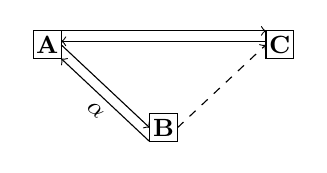
\begin{tikzpicture}[scale=1]
  
  \small
  
  \newcommand\X{210/5pt};
  \newcommand\Y{30pt};

  
  \draw[fill=white] (0*\X, 0*\Y) node{\textbf{A}} +(-5pt, -5pt) rectangle +(5pt, 5pt);
  % \draw (-5+0*\X, 0*\Y) node[left]{$E: \{a:2\}$};
  \draw[fill=white] (1*\X, -1*\Y) node{\textbf{B}} +(-5pt, -5pt) rectangle +(5pt, 5pt);
  % \draw (1*\X, -5-1*\Y) node[below]{$E: \varnothing$\vphantom{$\{$}};
  \draw[fill=white] (2*\X,  0*\Y) node{\textbf{C}} +(-5pt, -5pt) rectangle +(5pt, 5pt);
  % \draw (5+2*\X, 0*\Y) node[right]{$E: \varnothing$\vphantom{$\{$}};
  % \draw (5+2*\X, 0*\Y) node[right]{\phantom{$E: \{a:1\}$}};
  
  \draw[->](5+0*\X, 0*\Y) -- (-5+1*\X, -1*\Y); %% A->B
  \draw[<-](5+0*\X, -5+0*\Y) -- node[sloped, below]{$\bm{\alpha}$} (-5+1*\X, -5-1*\Y); %% A<-B
  
  \draw[->](5+0*\X, 5+0*\Y) -- (-5+2*\X, 5+0*\Y); % A->C
  \draw[<-](5+0*\X,  1.25+ 0*\Y) -- (-5+2*\X,  1.25+ 0*\Y); % A<-C
  
  \draw[->,dashed](5+1*\X, -1*\Y) -- (-5+2*\X, 0*\Y); %% B<-C
  % \draw[->, dashed](5+1*\X, -5-1*\Y) -- (-5+2*\X, -5+0*\Y); %% B->C



\end{tikzpicture}}
    \hspace{10pt}
    \subfloat[Part B][Process~A receives $\alpha$ and routes it to Process~C.]
    {\input{input/figsolveB.tex}}
    \hspace{10pt}
    \subfloat[Part C][Process~C receives $\alpha$ and answers by sending $\beta$ 
    to Process~B using Process~A as mediator. Then, Process~C broadcasts
    $c_1$ and registers it in $B_\alpha$.]
    {\input{input/figsolveC.tex}}
    \hspace{10pt}
    \subfloat[Part D][Process~A receives $\beta$ and routes it to Process~B. 
    Process~A receives $c_1$ and forwards it to both its neighbors.]
    {\input{input/figsolveD.tex}}
    \hspace{10pt}
    \subfloat[Part E][Process~C receives and discards $c_1$. 
    Process~B receives $c_1$ and forwards it to its neigbhor.
    Process~B reiceves $\beta$ and replies $\pi$ to Process~C using Process~A 
    as mediator. Process~B broadcasts $b_1$ and registers it in $B_\beta$.]
    {
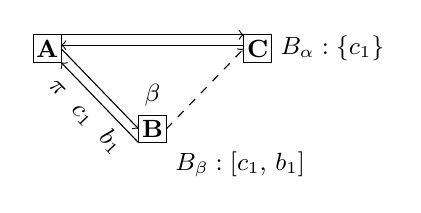
\begin{tikzpicture}[scale=1]
  
  \small
  
  \newcommand\X{190/5pt};
  \newcommand\Y{29pt};

  
  \draw[fill=white] (0*\X, 0*\Y) node{\textbf{A}} +(-5pt, -5pt) rectangle +(5pt, 5pt);
  % \draw (-5+0*\X, 0*\Y) node[left]{$E: \{a:2\}$};
  \draw[fill=white] (1*\X, -1*\Y) node{\textbf{B}} +(-5pt, -5pt) rectangle +(5pt, 5pt);
  \draw (1*\X, 5-1*\Y) node[above]{$\beta$};
  \draw (5+ 1*\X, -5-1*\Y) node[below right]{$\bm{B_\beta: [c_1,\,b_1]}$};
  % \draw (1*\X, -5-1*\Y) node[below]{$E: \varnothing$\vphantom{$\{$}};
  \draw[fill=white] (2*\X,  0*\Y) node{\textbf{C}} +(-5pt, -5pt) rectangle +(5pt, 5pt);

  \draw (5+2*\X, 0*\Y) node[right]{$B_\alpha: \{c_1\}$};

  % \draw(2*\X, 5+0*\Y) node[above]{$\alpha$};
  % \draw (5+2*\X, 0*\Y) node[right]{$B_\alpha: \{c_1\}$};
  
  \draw[->](5+0*\X, 0*\Y) -- (-5+1*\X, -1*\Y); %% A->B
  \draw[<-](5+0*\X, -5+0*\Y) -- node[sloped, below]{$\bm{\pi}$~~$c_1$~~$\bm{b_1}$} (-5+1*\X, -5-1*\Y); %% A<-B
  
  \draw[->](5+0*\X, 5+0*\Y) -- (-5+2*\X, 5+0*\Y); % A->C
  \draw[<-](5+0*\X,  1.25+ 0*\Y) -- (-5+2*\X,  1.25+ 0*\Y); % A<-C
  
  \draw[->,dashed](5+1*\X, -1*\Y) -- (-5+2*\X, 0*\Y); %% B<-C
  % \draw[->, dashed](5+1*\X, -5-1*\Y) -- (-5+2*\X, -5+0*\Y); %% B->C



\end{tikzpicture}
}
    \hspace{10pt}
    \subfloat[Part F][Process~A receives $c_1$ and discards it.
    Process~A receives $\pi$ and routes it to Process~C. Process~A receives $b_1$
    and forwards it to its neighbors. Process~C broadcasts $c_2$ and registers it 
    in $B_\alpha$]
    {
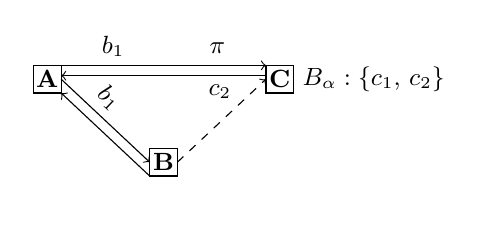
\begin{tikzpicture}[scale=1]
  
  \small
  
  \newcommand\X{210/5pt};
  \newcommand\Y{30pt};

  
  \draw[fill=white] (0*\X, 0*\Y) node{\textbf{A}} +(-5pt, -5pt) rectangle +(5pt, 5pt);
  % \draw (-5+0*\X, 0*\Y) node[left]{$E: \{a:2\}$};
  \draw[fill=white] (1*\X, -1*\Y) node{\textbf{B}} +(-5pt, -5pt) rectangle +(5pt, 5pt);
  % \draw (1*\X, 5-1*\Y) node[above]{$\beta$};
  \draw (5+ 1*\X, -5-1*\Y) node[below right]{\phantom{$B_\beta:\{b_1\}$}};
  % \draw (1*\X, -5-1*\Y) node[below]{$E: \varnothing$\vphantom{$\{$}};
  \draw[fill=white] (2*\X,  0*\Y) node{\textbf{C}} +(-5pt, -5pt) rectangle +(5pt, 5pt);
  % \draw(2*\X, 5+0*\Y) node[above]{$\alpha$};
  \draw (5+2*\X, 0*\Y) node[right]{$B_\alpha: \{c_1,\, c_2\}$};
  
  \draw[->](5+0*\X, 0*\Y) -- node[above, sloped]{$b_1$~~~~} (-5+1*\X, -1*\Y); %% A->B
  \draw[<-](5+0*\X, -5+0*\Y) -- (-5+1*\X, -5-1*\Y); %% A<-B
  
  \draw[->](5+0*\X, 5+0*\Y) -- node[above]{$b_1$~~~~~~~~~~$\pi$} (-5+2*\X, 5+0*\Y); % A->C
  \draw[<-](5+0*\X,  1.25+ 0*\Y) -- (-5+2*\X,  1.25+ 0*\Y) node[below left]{$c_2$~~~~}; % A<-C
  
  \draw[->,dashed](5+1*\X, -1*\Y) -- (-5+2*\X, 0*\Y); %% B<-C
  % \draw[->, dashed](5+1*\X, -5-1*\Y) -- (-5+2*\X, -5+0*\Y); %% B->C



\end{tikzpicture}}
    \hspace{10pt}
    \subfloat[Part G][Process~A receives $c_2$ and forwards it to its neighbors.
    Process~B broadcasts $b_2$ and registers it in $B_\beta$. Process~C receives
    $\pi$ and replies $\rho$ to Process~B using Process~A as mediator. Then it 
    receives and forwards $b_1$. Then it broadcasts $c_3$. It registers $b_1$ 
    and $c_3$ in $B_\pi$.]
    {\input{input/figsolveG.tex}}
    \hspace{10pt}
    \subfloat[Part H][Process~A receives and discards $b_1$. 
    Process~A receives and routes $\rho$ to Process~B. 
    Process~A receives and  forwards $b_2$ then $c_3$. Process~B receives, forwards, 
    and registers $c_2$. Then Process~B receives $\rho$ and sends $B_\beta$ to
    Process~C using the new link.]
    {\input{input/figsolveH.tex}}
    \hspace{10pt}
    \subfloat[Part I][Once Process~A sent $B_\beta$, the new link is safe.
    Process~C receives $B_\beta$. Process~C does not deliver $b_1$ and $c_2$, for it
    already delivered them. Process~C delivers $b_2$ and
    expects another copy from Process~A, for it constitutes a new message. 
    Process~C expects to eventually receive $c_3$ from Process~B.]
    {
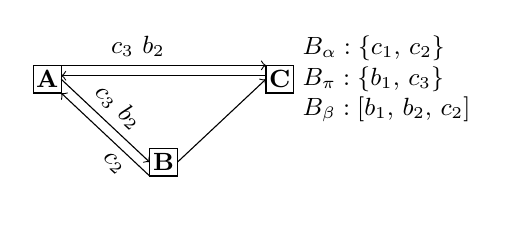
\begin{tikzpicture}[scale=1]
  
  \small
  
  \newcommand\X{210/5pt};
  \newcommand\Y{30pt};

  
  \draw[fill=white] (0*\X, 0*\Y) node{\textbf{A}} +(-5pt, -5pt) rectangle +(5pt, 5pt);
  % \draw (-5+0*\X, 0*\Y) node[left]{$E: \{a:2\}$};
  \draw[fill=white] (1*\X, -1*\Y) node{\textbf{B}} +(-5pt, -5pt) rectangle +(5pt, 5pt);
  % \draw (1*\X, 5-1*\Y) node[above]{$\rho$};
  \draw (5+ 1*\X, -5-1*\Y) node[below right]{\phantom{$B_\beta: [b_1,\,b_2,\,c_2]$}};
  % \draw (1*\X, -5-1*\Y) node[below]{$E: \varnothing$\vphantom{$\{$}};
  \draw[fill=white] (2*\X,  0*\Y) node{\textbf{C}} +(-5pt, -5pt) rectangle +(5pt, 5pt);
  % \draw(2*\X, 5+0*\Y) node[above]{$\pi$};
  \draw (5+2*\X, 0*\Y) node[right, align=left]{$B_\alpha: \{c_1,\, c_2\}$\\$B_\pi: \{ b_1,\, c_3 \}$\\$B_\beta: [b_1,\,b_2,\,c_2]$};
  
  \draw[->](5+0*\X, 0*\Y) -- node[sloped, above] {$\bm{c_3}$ $b_2$} (-5+1*\X, -1*\Y); %% A->B
  \draw[<-](5+0*\X, -5+0*\Y) -- node[sloped, below]{~~~~~ $c_2$} (-5+1*\X, -5-1*\Y); %% A<-B
  
  \draw[->](5+0*\X, 5+0*\Y) -- node[above]{$c_3$ $\bm{b_2}$ ~~~~~~} (-5+2*\X, 5+0*\Y); % A->C
  \draw[<-](5+0*\X,  1.25+ 0*\Y) -- (-5+2*\X,  1.25+ 0*\Y); % A<-C
  
  \draw[->](5+1*\X, -1*\Y) -- (-5+2*\X, 0*\Y); %% B<-C
  % \draw[->, dashed](5+1*\X, -5-1*\Y) -- (-5+2*\X, -5+0*\Y); %% B->C
\end{tikzpicture}}\\
    %\hspace{10pt}
    \subfloat[Part J][Process~C categorizes each message of $B_\beta$ using its two 
    own buffers $B_\alpha$ and $B_\pi$.]
    {
\begin{tikzpicture}[scale=0.88]

  \small
  
  \newcommand\X{210/5pt};
  \newcommand\Y{30pt};
  
  \newcommand\RADX{3.5};
  \newcommand\RADY{2};

  \newcommand\OFFX{15pt};

  \draw[pattern=north west lines, pattern color=blue!30] (0*\X, 0pt) circle [x radius=\RADX*\X, y radius = \RADY*\Y];
  \draw[pattern=north east lines, pattern color=red!35] (\RADX*\X, 0pt) circle [x radius=\RADX*\X, y radius = \RADY*\Y];

  \draw (0*\X, 0pt) circle [x radius=\RADX*\X, y radius = \RADY*\Y];
  \draw (0*\X, \RADY*\Y) node[below, align=center]{\textbf{\COLOR{blue!80!black!70}{\uline{Delivered by}}}\\\textbf{\COLOR{blue!80!black!70}{\uline{Process~B}}}};

  \draw (\OFFX-\RADX*\X, 0pt) node[right, align=left] {
    \textbf{\COLOR{blue!80!black!70}{To deliver:}}\\%\tiny
    $B_\beta \setminus B_\alpha \setminus B_\pi$\\\tiny
    $[c_1,\,b_1,\,b_2,\,c_2]\setminus\{c_1,\,c_2\}\setminus\{b_1,\,c_3\}$\\\tiny
    $[b_1,\,b_2] \setminus \{b_1,\,c_3\}$\\%\tiny
    \COLOR{blue!80!black!70}{$\bm{[b_2]}$}
  };
  \draw (-\OFFX+2*\RADX*\X, 0pt) node[left, align=right] {
    \textbf{\COLOR{red!80!black!70}{To expect from B:}}\\%\tiny
    $B_\pi \setminus B_\beta$\\\tiny
    $\{b_1,\,c_3\} \setminus [c_1,\,b_1,\,b_2,\,c_2]$\\\tiny
    \\
    \COLOR{red!80!black!70}{$\bm{\{c_3\}}$}
  };
  \draw (0.5*\RADX*\X, 0pt) node[align=center] {
    \textbf{\COLOR{purple}{To ignore:}}\\%\tiny
    $B_\beta \wedge (B_\alpha \cup B_\pi)$\\\tiny
    $[c_1,\,b_1,\,b_2,\,c_2] \wedge (\{c_1,\,c_2\} \cup \{ b_1,\,c_3\})$\\\tiny
    $[c_1,\,b_1,\,b_2,\, c_2] \wedge \{b_1,\, c_1,\, c_2,\, c_3 \}$\\%\tiny
    \COLOR{purple}{$\bm{\{c_1,\, b_1,\, c_2 \}}$}
  };
  \draw (\RADX*\X, 0pt) circle [x radius=\RADX*\X, y radius = \RADY*\Y];
  \draw (\RADX*\X, \RADY*\Y) node[below, align=center]{\textbf{\COLOR{red!80!black!70}{\uline{Delivered by}}}\\\textbf{\COLOR{red!80!black!70}{\uline{Process~C}}}};
\end{tikzpicture}
}
    \caption{\label{fig:solve}Using buffers and control messages, \RPCBROADCAST 
      provides reliable causal broadcast.}
  \end{center}
\end{figure*}



Similarly to \PCBROADCAST, the size of buffers may increase unbounded when
intermediate processes are faulty. Control messages never reach their
destination. \PCBROADCAST handles such crashes using a timeout and retry
policy. Such strategy fits \RPCBROADCAST.  \TODO{Receiving may ignore all
  incoming messages.}


\subsection{Complexity}
\label{subsec:complexity}

In this section, we analyze the complexity of \RPCBROADCAST in terms of
broadcast message overhead, delivery execution time, local space consumption,
and number of control messages. 

\noindent The \textbf{broadcast message overhead} is constant $O(1)$, for it
only piggyback the control information to ensure reliable FIFO links.

\noindent The \textbf{delivery execution time}, i.e., the time complexity of the
receipt function, is constant $O(1)$, for it only checks if the message should
be discarded or delivered. \TODO{Maybe O(P).}

\noindent The \textbf{local space consumption} depends on the size of
buffers. There are 4 buffers in total. $W$ is the size of buffers related to
reliable FIFO links. A link may delay the delivery of messages to await some
preceding messages. $B_\beta$ is the size of buffers of messages that increases when
the process adds a neighbor in its out-view, and decreases when a link become
safe. $B_\alpha$ and $B_\pi$ are the size of buffers of messages that increases
when the process gets added as neighbor, and decreases when a links in its
in-view become safe. The space complexity of \RPCBROADCAST is
$O(W  + B_\alpha + B_\beta + B_\pi)$. It grows and shrinks depending on the dynamicity
of the system. If the system becomes static, the space complexity of
\RPCBROADCAST is $O(W)$. If the system becomes quiescent, the space complexity
of \RPCBROADCAST is $O(B_\alpha+ B_\beta + B_\pi)$.  If the system becomes both
static and quiescent, \RPCBROADCAST does not consume
space. 

\noindent The overhead in terms of \textbf{number of control messages} per added
link in an out-view varies from $6$ to $4N^2$ depending on the overlay
network. It achieves $6$ messages when Process~A adds Process~B using Process~C
as mediator, and Process~B has Process~A in its out-view. It achieves $4N^2$
when Process~A adds Process~B without knowledge of any route. Process~A and
Process~B fall back to reliable broadcast to disseminate control
messages. \TODO{$N$ is the size of the network.}

Overall, this analysis shows that \RPCBROADCAST proposes an advantageous
tradeoff when the overlay network allows routing between the process that adds
the neighbor and the latter. Fortunately, a wide range of peer-sampling
protocols building overlay networks rely on close neighbor-to-neighbor
interactions to establish links (\REF). An \RPCBROADCAST built on top of these
peer-sampling protocols achieves $8$ control messages per added link. Several
other peer-sampling protocols build addressable overlay networks which allows
routing with a logarithmic number of hops compared to the actual network size
(\REF). An \RPCBROADCAST built on top of these peer-sampling protocols achieves
$O(4\log(N))$ control messages per added link.

Assuming such overlay network, \RPCBROADCAST constitutes a lightweight and
efficient middleware for reliable broadcast and causal broadcast in large and
dynamic distributed systems. As consequence, these broadcast can run in large
and dynamic systems even on most humble devices such as Raspberry Pi's.


%%% Local Variables:
%%% mode: latex
%%% TeX-master: "../paper"
%%% End:
